
\chapter{Reunions}

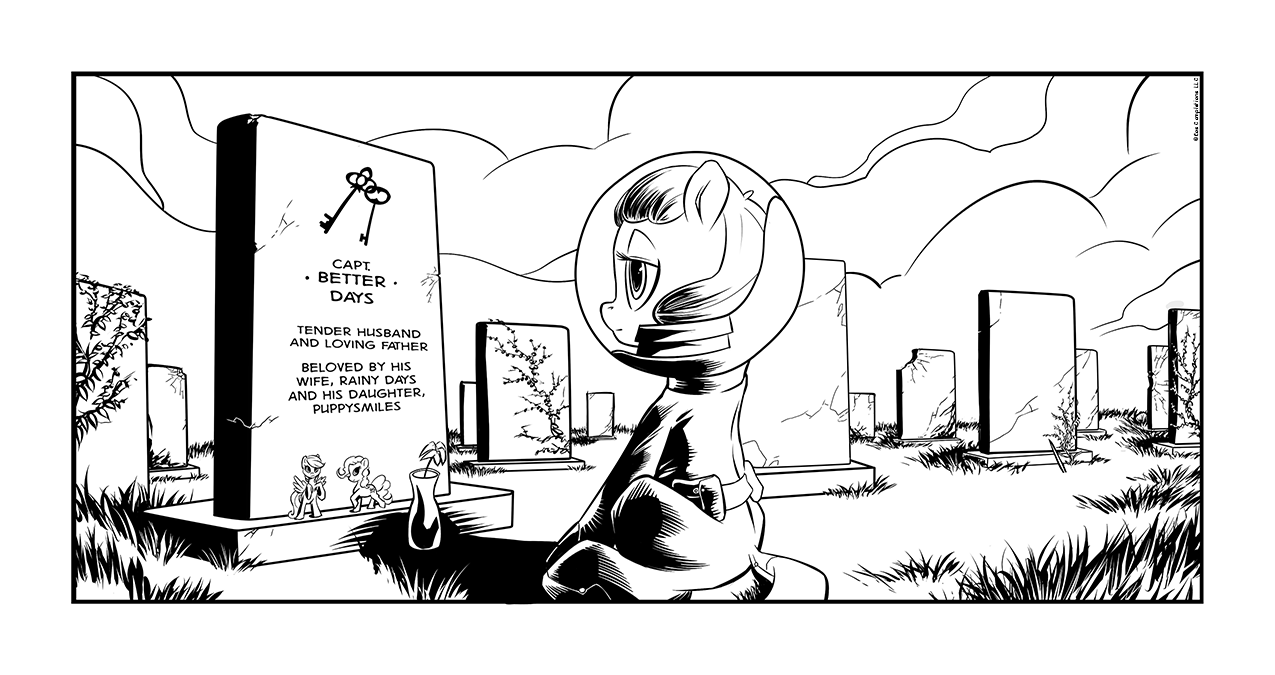
\includegraphics[width=0.9\linewidth]{image16.png}

\begin{intro}
We're getting the band back together
\end{intro}


\rtpr{'Sup, ponies. I can't believe he really did that! He took that piece of crap he calls a rifle and just flew away. That feather head! While I was sleeping! Hey L.P., if you are listening to this, shove that rifle up your ass!}

The radio paused for a moment, the feminine voice that had been talking didn't seem sad or worried, just angry.

\rtpr{All right ponies, the show must go on! DJ Good Stuff here, and you are listening to Radio 52, at least until I collapse because a certain pony left me here all alone with a show that is never supposed to stop! Okay, new rules: I'll be airing during daytime, and you'll get only music during night, because I'm not immortal and I need to sleep. And if anypony wants to drop by and do some talking while I'm asleep, just knock at the door. You know where we are.}

The sound of paper shuffling filled another pause.

\rtpr{All right, remember that I can operate that damn shortwave radio too, so don't stop sending news, especially regarding the situation in Ironworks. And speaking of news, the Memorial has been deserted, and the ponies are moving north, toward Broccoli. All the caravans still moving between Broccoli and Emerald Shores should head north and try to reach Rust Manor. I repeat, head north towards Rust Manor! Don't stop at Broccoli, because it's too near to the war zone.}

\rtpr{Fuck, I hate giving the news. If anything else comes in I'll let you know, otherwise you'll get music all day long. Remember, music means no news and no news is actually good news. Have some angry music because I'm angry and give Lonesome a buck in the head if you see him.}

\begin{music}
		Say your prayers, little one,
	
		Don't forget, my son,
	
		To include every pone.
	
		Tuck you in, warm within,
	
		Keep you free from sin,
	
		`til the sandmare she comes
\end{music}

\horizonline

\englishdaytimeplace{13}{4:00 A.M.}{The Memorial northern picnic area, Big 52 S Branch}

In the distance, far ahead of Puppysmiles, stood another little town, little more than a group of shacks built around a very large statue that depicted a group of ponies hoisting an Equestrian banner. The marble monument was remarkably well conserved, and its enormous size made it possible to see even from several kilometers away. On her way south, she met several groups of ponies with carts loaded with everything. She tried to socialize with them, but they simply kept moving, mostly ignoring Puppy except for a couple of foals who waved back from a cart. Entire families were fleeing, leaving their homes and trying to reach safety behind the walls of larger and better guarded settlements.

She was now staring at the monument with a puzzled expression. ``Ah, Mister Voice, are we near to dad's place?''

{\mt ``Analyzing. Actual position is Equestria: Fallen Soldiers Memorial, northern picnic area. Location of your male parent is currently unknown.''}

Puppy tilted her head, studying the surroundings. ``Yes, I remember this place! That big road sign with the Pinkie Pie face and\dots'' She left the road, galloping over a low hill and finding herself in the middle of a group of tables and rusty abandoned barbecues. ``This is dad's place! Dad is near! Let's go!''

Puppy galloped further away from the road, heading for a group of hills to the west. The low hills were still far from here, approximately four or five kilometers away from the Memorial, but even from this distance it was possible to see that they were dotted with white stones, each spaced evenly apart.

As she ran toward the distant hills, Puppy passed by a dead tree. Once upon a time it must have been a proud oak, but all that was left now was just a blackened skeleton, its trunk scorched and its branches bare.

\rcpr{``I want more apple pie!''}

\rcpr{The grass was green and birds were singing among the leaves. The sky was blue and everything was so nice.}

\rcpr{``Don't eat too much Puppy, we still need to go to dad's place, remember? If you eat too much you'll get sleepy, and you don't want to be sleepy when we go visiting Dad, right?''}

\rcpr{``But Mom, he's never there! We went a lot of times and he was always away! Will he be there this time?''}

\rcpr{``I\dots I don't know, Puppy, but you can leave him flowers, so he will find them and know that you love him, okie dokie?''}

\rcpr{A couple of colts chased each other, disappearing behind a hill. There were ponies playing and ponies having lunch. Everypony was having a good time.}

\rcpr{``I got a better thing this time! Look!''}

\rcpr{``Oh, but Puppy, that's a toy of yours! Are you sure you want to leave it here?''}

\rcpr{``Yush! So when Dad will be back he will play with it and won't feel lonely! Besides, he will return it to me when he comes back home again!''}

\rcpr{``\dots''}

\rcpr{The distant sound of laughter filled the silence between mother and daughter.}

\rcpr{``Mom? Why are you crying?''}

She stopped for a moment, looking at the big tree and trotting around it. She could clearly remember having a picnic in this place not earlier than in spring. Where had everything gone? Oh well, she knew that trees sometimes lose their leaves because Mom had told her so and since there wasn't even grass on the ground it was just fitting. She trotted away toward the cemetery.



\horizonline

\englishdaytimeplace{13}{6:00 A.M.}{Interequestrian 52 War Cemetery, Big 52 S Branch}

The tombs were all similar, consisting of small marble stones on which were engraved a name, a date, a cutie mark and a few short words. Some stones were white and other stones were black, but when Puppy asked to her mom why they were different she simply replied that the ponies napping there were more important than the others. Puppy didn't like that reply, since Dad was a very important pony but he only had a white stone; so she decided to bring him some more flowers, just to show him that she was super sure he was the best dad ever.

{\mt ``Warning. Receiving distress radio signal. Distance from the source: two hundred meters. Signal identified: Device 009. Warning. Receiving new distress radio signal. Distance from the source: two hundred and fifty meters. Signal identified: Device 020.''}

Puppy tilted her head, confused. ``Wut? New radio music? I hope it's not like the last time when there was just a stoopid pony saying endlessly `help me, we're doomed' and all those silliness.''

{\mt ``Negative. These are Ministry of Peace distress signals from other MK VI Suits. Receiving a third signal on a distance of two hundred and thirty meters. Signal identified: Device 013.''}

She sighed. ``Look, if it's not music I don't care. Now let's go find Dad, maybe he's back and we will go find Mom together.'' With these words, Puppy headed toward a low hill with the statue of an alicorn on top.

The hill was surrounded by a low fence with several marble arches that led inside that area of the cemetery. A large main battle tank stood in front of the arch Puppy was going through. A brass plaque in front of the war machine explained that in this part of the graveyard were buried the fallen soldiers from the Third Armored Company--Steel Flanks. There were also some commemorative words and a brief statement that explained how tanks nowadays weren't widely used on the front because of the new technological breakthroughs, and that this decommissioned machine had been left here to safeguard its sleeping brothers.

Puppy had been here more than once, so she already knew where to go and headed toward a specific grave. Seeing that the place was deserted, Puppy sighed and sat in front of the white stone.

The cutie mark of a couple of keys was engraved on the marble surface, together with some writing:

\begin{center}
	Captain \quad Better Days

	Tender husband and caring father.

	\medskip

	Beloved by
	
	his wife \quad Rainy
	
	and his daughter \quad Puppysmiles.
\end{center}

% NOTE: Modifine style

The date was mostly unreadable, but it didn't matter very much to Puppy, since she was mostly interested in the grave itself. On the small mound sat an empty vase and a couple of plastic figures. The vase once contained flowers, but now it was just filled with murky water and covered in mold, but the plastic figures still stood on the grave, looking back at Puppy. They were two molded plastic ponies, like those that were put into cereal boxes. The first figure was a miniature Pinkie Pie, while the other was of Rainbow Dash.

Puppy sighed. ``He didn't take them\dots Why does he never takes what I leave here? I was sure that he loved Pinkie Pie and Rainbow Dash!'' Touching the plastic blue pegasus with a hoof, she continued, ``Stoopid Dad; if he was a little more at home, Mommy could be happy\dots''

Oh well, Mom explained plenty of times that it was okay if he didn't come home and that she wasn't mad at him. She wasn't completely convinced, but something in her mother's eyes told her that she just had to accept that explanation. From the day Mom got angry because Puppy didn't want to come home until dad came back with them too, she decided that she didn't want to see her mother cry and scream like that. So she decided to play along and leave something in this place every time she came here, hoping that one day Dad would realize that she and Mom still loved him and maybe he would finally come back.

Puppy cleared her voice and stated, ``Everything.''

{\mt ``Warning. The inventory management spell is not devised to operate more than one object at a time. Opening fast inventory scrolling by alphabetical order. State `next' when you have finished examining an object and need to move on. State `stop' or `exit' when you want to close this application and restore usual inventory management program.''}

An ashtray floated in front of puppy. ``Next!'' Another ashtray appeared. ``Next!'' Yup, ashtray. ``Next!'' Again, an ashtray ``Next!'' Puppy usually scooped up every single shiny object she found on her way, so this was going to take a while.


\horizonline

\englishdaytimeplace{13}{7:00 A.M.}{Interequestrian 52 War Cemetery, Big 52 S Branch}

``Next!'' The twentieth fork was stowed back into Puppy's bags and the sorry, dripping remains of Fuzzy Ball floated in front of the foal. ``Ne---no wait! Fuzzy!'' Grabbing the dead parador cub, a disgusting green goo oozed from the cracks in its carapace. The dead creature had lost all of its legs and only had a single wing left, while the eyes at some point started to decompose and were now just another grossly rotting detail on that thing.

``You don't seem very healthy today, Fuz. What happened?'' Puppy studied the dead creature for a moment, trying and failing to determine what was wrong with it. ``Ah, Mister Voice, is Fuzzy Ball ill?''

{\mt ``Negative. Fuzzy Ball is deceased and in an advanced state of decay.''}

Puppysmiles frowned. She had learned from experience that difficult words usually weren't good news. ``Ah, this means she is very tired?''

{\mt ``Negative. This means she is falling apart. Losing pieces. Disintegrating.''}

``What?'' Puppy cocked her head, alarmed. ``Losing pieces? But Fuz needs her pieces to be okay!'' She gave a second look at the dead critter. ``Besides, it seems to me that she doesn't lack any pieces.''

{\mt ``Advice. Check twice. The creature has lost three wings and all its legs. Moreover, its carapace is rotting and has broken in several places due to the poor condition in which it has been transported.''}

``Transported? You mean that Fuzzy is getting worse because I am taking her along with me? But that's terrible!''

This was a chance that even an automated voice with no real intelligence could be able to exploit.

{\mt ``Affirmative. The corpse is decomposing faster mostly because of you insisting on taking it along. Abandoning the corpse immediately is highly recommended.''}

Puppy hesitated. ``Leaving Fuzzy here? But---but she will be alone! There's nothing here, there's only---'' She stopped talking, looking straight at her father's grave. ``Maybe Dad could take care of her.'' Puppy didn't seem enthusiastic about that idea, still it seemed so obvious.

{\mt ``Elaborating. Leaving a deceased pet in the custody of a deceased parent is\dots Error, cannot compute. Please reformulate.''}

``Reform me late? What are you saying again, you silly voice? I'm trying to being serious here!''

{\mt ``Re-elaborating. It is impossible to identify a logical pattern. An external counselor is strongly advised.''}

Puppy snapped, starting to lose her legendary patience. ``Stop talking nonsense! Call me somepony more competent or we'll end up arguing again!'' She put her hooves on her helmet, as if she was rubbing her head. ''Really, living with you can be a pain sometimes.''

Watcher's staticky voice interrupted the foal-machine quarrel. ``Puppy? What are you doing in this place? It's dangerous!''

Turning toward the voice, Puppy found a spritebot floating to her left, but this time she couldn't smile at him. ``Oh, it's you, Questioner---''

``Watcher\dots''

``---Whatever. This isn't a good moment, could you please come back some other time?''

He hesitated before replying. ``Sure, but I wanted to warn you. This place is not good for you. It's filled with, uh, bad things that you must not see. Please, before I go, promise me that you will get away from here immediately.''

Puppy snorted in frustration. ``I can't. I need help with Fuzzy Ball, but Mister Voice is not helping at all!'' With these words, she showed her dead parador to the spritebot.

``Gah! But that thing is rotting! No please, what is that? Don't tell me! Puppy, throw that thing away!''

``What? But Fuzzy Ball is my very best pet friend! I love her and she loves me and we are having lot of adventures together! I don't want to abandon her\dots'' She hesitated, looking away. ``But\dots''

``But?'' pressed Watcher, since Puppy didn't seem eager to end the sentence and still hugged the corpse.

``But she is ill, and Mister Voice says that she must rest! I could leave her with my dad, but it seems wrong. I didn't even ask him if I could keep her and---''

``Your dad? You know where your dad is and you are still trotting alone through the Wasteland?'' His voice was growing with indignation. ``What kind of a father could ever leave his---'' Watcher stopped abruptly, finally noticing the name on the grave that Puppy was sitting in front of. ``Oh\dots This keeps getting better\dots''

She went on, ``I know that I should have asked before taking a pet with me but, but\dots'' She sobbed. ``But I only wanted a friend to stay with me all the time! Not a weird voice that always tells me what to do, or a stoopid chicken that comes and goes! Fuzzy never leaves me alone and keeps me company! We were having lot of fun together and I protected her from the pet eaters and she never goes away and\dots''

Puppy paused, looking at the spritebot. ``And now she is ill and she loses pieces! Mister Voice says she has less wings than before. I'm not good with numbers, but it seems that he's right! I don't want to leave her, but I don't want her to be ill because of me. I don't know what to do!''

``Ah, and what did Mister Voice say?''

Puppy snorted. ``Nothing! He is talking nonsense since I started asking him! Then I had this idea of letting Fuzzy stay here with Dad to see if she gets better, but I don't know if Dad will like her or if he will be angry and, well, I'm not sure Dad will come here, because he is never here when I come, and even if Mom says he loves me, I can't figure why he always avoids me!'' She waved her hooves around, as if she couldn't stand still while she was expressing her concern. ``So maybe he will hate Fuzzy Ball and then she will be sad, but I can't take her with me because she's losing pieces, and losing pieces is bad!''

Watcher hesitated, trying hard to disentangle the knot of feelings and words that Puppy was bombarding him with. ``Well, um, what if I take Fuzzy with me? Just put her into this spritebot's cargo bay and I'll take care of the rest! Sound fair?''

Puppy tilted her head. ``You will make Fuz feel better? Really?''

``Sure, she can't get any worse anyway. I'll see what I can do, but now please, get away from this place, it's not good for you.'' With these words, a hatch opened on the spritebot's side, revealing a space large enough to house the dead critter.

She looked at the metallic stash, then at Fuzzy Ball and sighed. Hugging her pet one last time, she whispered her goodbye. ``Don't worry, Questioner is a pretty pony. When you get better we will play again together.'' Kissing Fuz goodbye through the helmet's glass, Puppy put the dead creature inside the spritebot, the hatch closing almost immediately.

``Don't worry about her, little one, she is going to a better place. Now, let's move away from here, it makes me sad, okay?''

She nodded, looking at her father's grave. ``Lily.'' A plastic flower floated in front of her and she put it on the ground before the marble stone. ``Sorry Dad, I have to go. But next time I'll stay a little more, okie dokie? I'll come here with Mom.'' Turning away from the grave, Puppy smiled at the spritebot. ``All right, I'm done.''

There was a pause before Watcher spoke again. ``You're a good filly, Puppy.''

Puppy and Watcher moved off along the road that headed away from the cemetery, towards the Memorial. The ponies on the large statue seemed to salute the fallen from across the distance, like an eternal link from those who had died fighting and those who were left, trying to win a war that in the end killed everypony.



\horizonline

\englishdaytimeplace{13}{7:15 A.M.}{The Memorial, Big 52 S Branch}

The Memorial was completely empty. While fleeing from the town the inhabitants had taken with them everything that wasn't nailed down and even a few nails that had come loose. By the time two ponies and a sealed crate were flown in by way of griffon, there was only dust and rust left to meet them.

``All right, we're here.'' Mister White jumped down from the griffon that was transporting him and stretched his legs. ``That was a long trip.'' He tipped his black hat. ``You lot can go back to Sun City.''

The first mercenary griffon nodded to him. ``Okay, boss, but are you sure you want us to leave?''

He snickered, looking at the other pony as he disembarked clumsily. ``Absolutely. This is family business, we just needed to get here fast, now your work is done.'' The griffon's expression was still uncertain. ``Oh, don't worry about your pay. If I don't come back, my son will take care of the company.''

The griffon shrugged and waved at the others. ``Okay, you heard the boss! Let's get out of here, lazy feathers!'' All three creatures took off the ground and headed north.

While Mister White watched the griffons flying away, Sage Brush dragged the heavy crate inside a small shack made of plastic sheets and large road signs, complaining all the way. ``We can't take all this stuff with us, Uncle White, it's too heavy!''

``Don't worry Sage, I'm planning to make camp here and then move fast, scouting the area. She can't be very far.''

``I still can't see why you decided to run all the way out there with just me for company when we could simply call the guys.''

``First of all, we had to get here fast and we can't airlift all those ponies and equipment in time. Moreover, Rust Manor is paying good caps for our mercenaries, and I don't see why we should lose earnings.'' Mister White tapped his chin, trying to find something else to add. ``Besides, we aren't going to face the Wild Herd; we will just get the foal and head back, easy peasy.''

Sage Brush sighed. ``Did anypony ever tell you that you're weird? I know she saved our rumps, but you already gave her a reward for that. I think this foal retrieving mission is suicide.'' He hesitated for a moment, his expression becoming thoughtful. ``Or do you know something I don't?''

Mister White enveloped a pair of binoculars with his telekinesis and scouted the surrounding hilltops. ``Well, let's just say that I asked some questions here and there and it seems that wherever that foal goes, things change for the better. This `ghost' must have some sort of lucky star watching over her, and I want to be there when the filly strikes again. There's a lot to gain from this story.''

Sage Brush waved a hoof, dubiously. ``And you say this because?''

``\dots Because I have a good feeling about it.''

Sage facehoofed. ``Great, so we are following a ghost because you have a doozy! Why am I coming with you?''

Mister White replied merrily, ``Well, because I'm your dear uncle and you owe me so many caps that you can't say no anyway.''

``I hate my life,'' groaned Sage Brush.

Mister White waved a hoof, asking for silence. ``Shut up! Somepony is coming from the hills, get the rifle.''

From their improvised sniping position, the two ponies observed the solitary figure trotting in town. It was covered in a dusty mantle and carried a long carbine on its back. The traveler's face was hidden under a hood, but from its neck hung a necklace of feathers and polished metal objects.

Sage Brush lowered his rifle, sighing in relief. ``Meh, it's just a farseer. Weird, what's a shaman doing this far from the desert?''

Mister White trotted out from the shack, leaving his rifle behind. ``We'll find that out soon.'' He galloped toward the newcomer and called out to him or her. ``Hey you! This place is empty. The road heading south is dangerous! You should turn your tail south and head north!''

The hooded pony stood for a moment, looking directly at Mister White before taking off her hood, revealing the face of an old unicorn mare. ``Oh, you are already here. Very well, now we have to wait for the others.''



\horizonline

\englishdaytimeplace{13}{7:30 A.M.}{The Memorial outskirts, Big 52 S Branch}

``So, Puppy, you never told me about that blue streak in your mane. How did you get it?'' The spritebot floated alongside Puppy as they slowly made their way from the cemetery and towards the Memorial. The graveyard gates were just a few hundred meters behind them.

``Ah, it was in Sun City, when Blue Voice told me all those meanie things. I don't remember very well, but at some point I went to sleep and when I woke up my mane was all fancy.''

``I see. You went to sleep, and woke up with your mane changed\dots and what did Mister Blue tell you?''

Puppy sighed. ``I already told you that! He said I was a robot and wanted to make a fool out of me, but I showed him that I was smarter. But that's an old story, since now we are friends.''

``Beg your pardon? You are friends now? Didn't you kill him with a mag pulse shell?''

Puppy giggled. ``Of course not, you silly Questioner! He is not a bullybot! He's just as stoopid as a colt! But when we met again and Creepy Voice bullied him, he said he was sorry so even if he pretends to be grumpy I know we're friends!''

``Creepy who now?'' The tiniest shadow of concern started dancing in Watcher's voice.

Puppy tapped at her helmet. ``You know, Creepy Voice! The one who lives in my head, talks weird and does a lot of cool stuff, but is a jerk?''

After a long pause, the spritebot replied. ``You mean Mister Voice, right?''

``Ah, nope. Mister Voice is a bit boring and talks nonsense, Creepy Voice is creepy but cool. She does stuff like opening doors and spanking bullybots.''

From the robot's speaker came a gasping sound. ``Ah, now I get it! It's an imaginary friend! Yeah, I remember something like that. Want some advice? Don't try blaming your friends for things you did. In the end it turns against you.''

Puppy tilted her head, a little confused. ``She didn't seem very imaginary. Ah, okie dokie?''

``Good filly, you always make me---''

\emph{BOOM!}

Watcher disappeared in a blaze of fire, right in front of Puppy's eyes.

She stepped back for a moment, trying to understand what was going on, then she noticed a large, squat metallic figure rolling over the top of a nearby hill and suddenly she knew the answer. ``Bullybots\dots''



\horizonline

\englishdaytimeplace{13}{8:00 A.M.}{The Memorial, Big 52 S Branch}

Mister White sat at a table inside the shack while Sage Brush finished cooking the oatmeal. ``All right, Long Ears, so when are these others ponies supposed to arrive?''

She shrugged, continuing to look outside the window. ``We should move by tomorrow evening. Many are coming, so much blood\dots''

Brush turned towards the farseer. ``Hey, old hag, we aren't going to fight! We're just here to get that foal and go back to Downtown. I don't care about your crazy visions.''

White waved a hoof at his nephew in an attempt to make him be quiet. ``Ah, you do the cooking, I do the talking. I think we already agreed on that.'' Turning back toward Long Ears, he went on. ``So, what did you see?''

She closed her eyes. ``In my dreams I've seen flames from the south, engulfing all in their path. In the blaze a pink shade kept struggling, the flames danced around her and they seemed to die for a moment as she passed them.'' She paused for a moment before continuing. ``As the fire continued to sweep north, the shade reached the end of the road and turned into darkness.''

Mister White frowned. ``Darkness? What do you mean with that?''

``A black wave that ran behind the fire, devouring it but not before it destroyed everything.'' She sighed. ``And when the darkness devoured the fire, nothing was left. The whole road was just an empty, abandoned place.''

``Well, that's boosting my motivation for sure!'' snapped Sage Brush. ``White, I say we go back to Downtown and leave this fucking place.''

White sighed, shaking his head and ignoring his nephew. ``So, why are we here?''

Long Ears looked away from the window. ``To stop the fire before it destroys everything, and then to reach the end of the road before the pink shadow does.''

``Pink shadow, you say? Why does this makes me think you are referring to Lonesome Pony's ghost?'' He was still talking when a distant explosion got his attention. ``Artillery\dots'' Looking outside the window, Mister White couldn't see any explosion, but it seemed to be quite distant, maybe seven or eight kilometers south east. 

Mister White trotted outside, listening for any more noises, but it was hard to tell if the sound he had heard was actually a distant gunfight or simply his imagination working too hard. ``Well, I guess that whatever it was, now it's gone. Let's get ins---'' A solitary figure was coming from the north, wearing a weathered duster and a leather hat.

He whistled. ``Hey, you! The place is deserted! Go back to Broccoli!'' Again, his voice hesitated when he recognized the newcomer. ``Oh, the old mummy\dots''

Molten Gold quickened his pace and smiled as he approached Mister White. ``Look who's here! White, of all the ponies I expected to meet, you are the last one! What are you doing in this outpost? Checking to see if there's something worth taking?''

He frowned. ``Oh, I'd never steal your job, old mummy. No, we are\dots checking on the situation with the Wild Herd. '' He paused for a moment, trying to read the ghoul's expression, but it wasn't an easy feat. ``So, what are you doing this near to the warzone? Some treasure hunting?''

Molten snickered. ``Something like that. Let's say that I sent a package south without realizing how dangerous it was. Now I'm trying to put a patch on that mistake.''

``This is something new! You being sorry for something! What happened, are you getting old?''

To Mister White's surprise, instead of replying immediately Molten Gold turned his eyes away, looking south. ``Well, yes. But I don't want a kid to die because of me being the usual me. I have a foal to save.''

Slowly, Mister White's expression of surprise changed into an amused smile, until he patted Molten on a shoulder. ``Welcome to the club. Come in, we have oatmeal and a hot mare inside.''



\horizonline

\englishdaytimeplace{13}{7:45 A.M.}{The Memorial southern picnic area, Big 52 S Branch}

Puppy galloped toward the big robot, with \emph{The Rock Of Destiny} floating at her side. ``Stop breaking my friends you stoopid bullybots!''

On the other side of Puppy's reckless charge stood an old, rusted but functional battle tank, with tracks, turret and everything else. A pony with a spiked mane was poking out of the turret hatch, taking his time as he stared at the solitary foal running toward them.

``Fuck the boss and his orders! Why should we hide in the south when we have a fucking tank! With this little baby we're unstoppable!

``Hey, Gray Matter, the yellow thing is running this way. How about some shooting practice on a moving target?'' With a laugh, the pony retreated inside the tank and closed the hatch. A few seconds later, the turret rotated to aim at the approaching Puppy.

Inside the tank, the pony with the spiked mane was snickering like mad. ``Come here, come here my little pony.''

``No wait!'' A mare with her mane completely cut off put a hoof on the gunner's flank. ``Let's try a different weapon, I want to see this one!''

``Shut up you cu---'' the stallion began scolding the mare, but at the last moment he noticed the big red button she was pointing at. ``Oh, yes! Yes I like it! Let's rocket it to the Moon!''

``You two idiots! Stop wasting time! Less talking, more shooting!'' Snapped the driver, an earth pony stallion.

The gunner snickered. ``Gee, you're such a whiner, Gray! Here, look at this!''

In the meantime, Puppy was a little more than halfway toward her target. Now that the big metal robot was near, she could see it had a large bulky body with a round head and a looooong nose. Oh, it was one of those carts full of teapots! Wait, they weren't bullybots, they were carts!

She stopped for a moment, sitting down and pondering on the nature of that thing. Okie dokie, what did she know? Usually there were ponies on the carts, but she couldn't see anyone on that one. Moreover, it broke Mister Questioner's robot, and this was a typical bullybot thing, so the odds were that it was a bullybot and not a cart, but to be perfectly sure she decided to go and ask.

In that moment, from the top of the tank's turret appeared a trail of white smoke that rocketed toward Puppy at a ludicrous speed. It was like a big funny firework! ``Tee-hee, look! A cloud maker!''

\emph{KABOOM!}

The rocket hit just behind Puppy, sending her flying towards the tank and leaving her in a small heap no more than fifty meters in front of it. Puppy's helmet was gone and the whole suit was peppered with holes. A thick curtain of pink mist was already forming around her while the suit read off its litany of damaged components.

``All right, he's a bullybot.'' Slowly, Puppy got back on her hooves and looked at the large metal monster that now stood in front of her. Her helmet was still missing and through the mist her face was blurry and hard to identify, except for two burning pink eyes that shone in the cloud, making the whole thing glow with an eerie light.

``Yeah! Eat it, yellow whatever!'' The pony with the spiked mane was laughing crazily, when the mare hit him in a flank again, causing him to snap in anger. ``What now, bitch?''

``Hey, Top Gun, I think it's standing up.''

``What the fuck is that? Gray Matter, stomp it!'' All right, the Wasteland was full of weird things and some of them could survive a missile in the face, but being trampled by a tank was a completely different level of overwhelming your enemy. The raider was sure that nothing could live through that.

The tank launched itself onward, aiming for Puppy, who was doing pretty much the same thing just from the opposite direction. When the two adversaries were almost on top of each other, Puppy jumped in the air, grappling the vehicle's frontal plate with her hooves and pedaling in the air with her hind legs.

``It's on the tank! Lucky Charm, go up and shoot it!'' The driver brought the tank to a sudden halt, trying to make her lose her grip, but while Puppy managed to stay holding on, the gunner was thrown forward, bashing his head against the cannon's loading mechanism and knocking him unconscious.

``Don't worry, I'm on it!'' The mare levitated a sub machine gun and opened the hull's frontal hatch, finding herself directly in front of the struggling foal and in the middle of the pink cloud. ``Say goodbye, critter!''

Puppy heard a voice in front of her, something that seemed pony-like, only she couldn't tell for sure. What she immediately recognized was the hail of bullets that pierced her head and her suit in several points, destroying what little of her helmet that had managed to reform. ``Stop it! Stoopid bullybot!''

A new surge of motivation gave Puppy the strength to haul herself completely onto the tank's hull, just to look at a hatch that was rapidly closing again. ``Hey, do you think you can keep me outside? I am Puppysmiles and I go wherever I want!''

She jumped on top of the turret, searching for something to hit with her faithful rock. Thick metal, some more metal, still metal, a glass thing---CRASH!---okay, more metal, an antenna---SDENG SDENG SDENG!---done, a box\dots ``Uh, a box! Okay, get ready for a spanking!'' Puppy loved that line from Creepy Voice, it sounded so cool!

Inside the tank, Lucky Charm was drowning in her own blood after breathing the pink mist, Top Gun was still unconscious and Gray Matter was trying his best to make the mare drink a healing potion. Everypony was simply too busy to worry about Puppy on the tank's roof that was hitting a missile rack with a stone.

This was more or less when Mister White heard the big explosion.



\horizonline

\englishdaytimeplace{13}{9:00 P.M.}{Interequestrian 52 War Cemetery, Big 52 S Branch}

It was much later when three figures approached the grave, not saying a word. All of them wore a MK VI suit, like Puppy's, but the ponies inside were a patchwork of rotting skin and bleached bones. In their burning pink eyes there was no sign of intelligence, nonetheless they stopped to study the hoofprints in front of the marble stone and followed the trail like hounds tracking their prey.

~\vfill

\begin{engnote}
		Level up! (15)
	
		New perk added: Hit the deck - What the fuck!? I was sure I hit her! Your Damage Threshold against explosives is raised by 25; enjoy tossing grenades on your feet.
\end{engnote}

